% CONVERGENCE_OVERVIEW.tex
% A one-page visual overview of the scqubits convergence-diagnostics subsystem:
% philosophy, workflow, verdicts, modes, channels, estimators, falsification
% checks, the composite/circuit/sweep hierarchy, and the report structure.
% Compile to a vector PDF:   pdflatex CONVERGENCE_OVERVIEW.tex
% Companion to CONVERGENCE_DEVELOPER_MANUAL.tex.

\documentclass[border=14pt]{standalone}
\usepackage{lmodern}
\usepackage{tikz}
\usetikzlibrary{positioning, arrows.meta, calc}

% ---- palette ---------------------------------------------------------------
\definecolor{ink}{HTML}{1F2933}
\definecolor{idea}{HTML}{0B7285}
\definecolor{flow}{HTML}{1864AB}
\definecolor{mode}{HTML}{5F3DC4}
\definecolor{chan}{HTML}{2B8A3E}
\definecolor{esti}{HTML}{E67700}
\definecolor{chek}{HTML}{C2255C}
\definecolor{hier}{HTML}{364FC7}
\definecolor{repo}{HTML}{495057}
\definecolor{vlikely}{HTML}{2F9E44}
\definecolor{vmaybe}{HTML}{74B816}
\definecolor{vmarg}{HTML}{F08C00}
\definecolor{vunver}{HTML}{868E96}
\definecolor{vdist}{HTML}{E03131}

% ---- geometry --------------------------------------------------------------
\def\colW{15.4cm}     % zone content width
\def\zoneH{6.0cm}     % uniform zone height
\def\colA{0}          % column x (north-west anchors)
\def\colB{17.2}
\def\colC{34.4}
\def\rowA{-2.7}       % row y (north-west anchors)
\def\rowB{-9.5}
\def\rowC{-16.3}

% ---- styles ----------------------------------------------------------------
\tikzset{
  zone/.style={
    draw=#1!70!black, line width=0.9pt, rounded corners=6pt,
    top color=#1!4, bottom color=#1!11, inner sep=10pt, anchor=north west, text=ink,
  },
  vchip/.style={
    rounded corners=2.5pt, fill=#1, text=white, font=\bfseries\scriptsize,
    inner xsep=4pt, inner ysep=2.5pt, anchor=base west,
  },
  pill/.style={
    rounded corners=3pt, draw=#1!70!black, fill=#1!12, text=#1!35!black,
    inner xsep=5pt, inner ysep=3pt, font=\bfseries\footnotesize, anchor=center,
  },
  fa/.style={-{Stealth[length=2.6mm]}, line width=1.1pt, draw=flow!75!black},
  gt/.style={font=\bfseries\footnotesize, text=ink!55, anchor=base west}, % ">" sep
}
\newcommand{\body}[1]{\begin{minipage}[t][\zoneH][t]{\colW}\setlength{\parskip}{2.2pt}\small #1\end{minipage}}
\newcommand{\zt}[2]{{\bfseries\textcolor{#1}{#2}}\par\vspace{2pt}}
\newcommand{\bk}[1]{\textcolor{ink!58}{\footnotesize #1}}
\newcommand{\cd}[1]{{\ttfamily\footnotesize #1}}
\newcommand{\bul}{\textcolor{ink!42}{\footnotesize$\bullet$}~}

\begin{document}
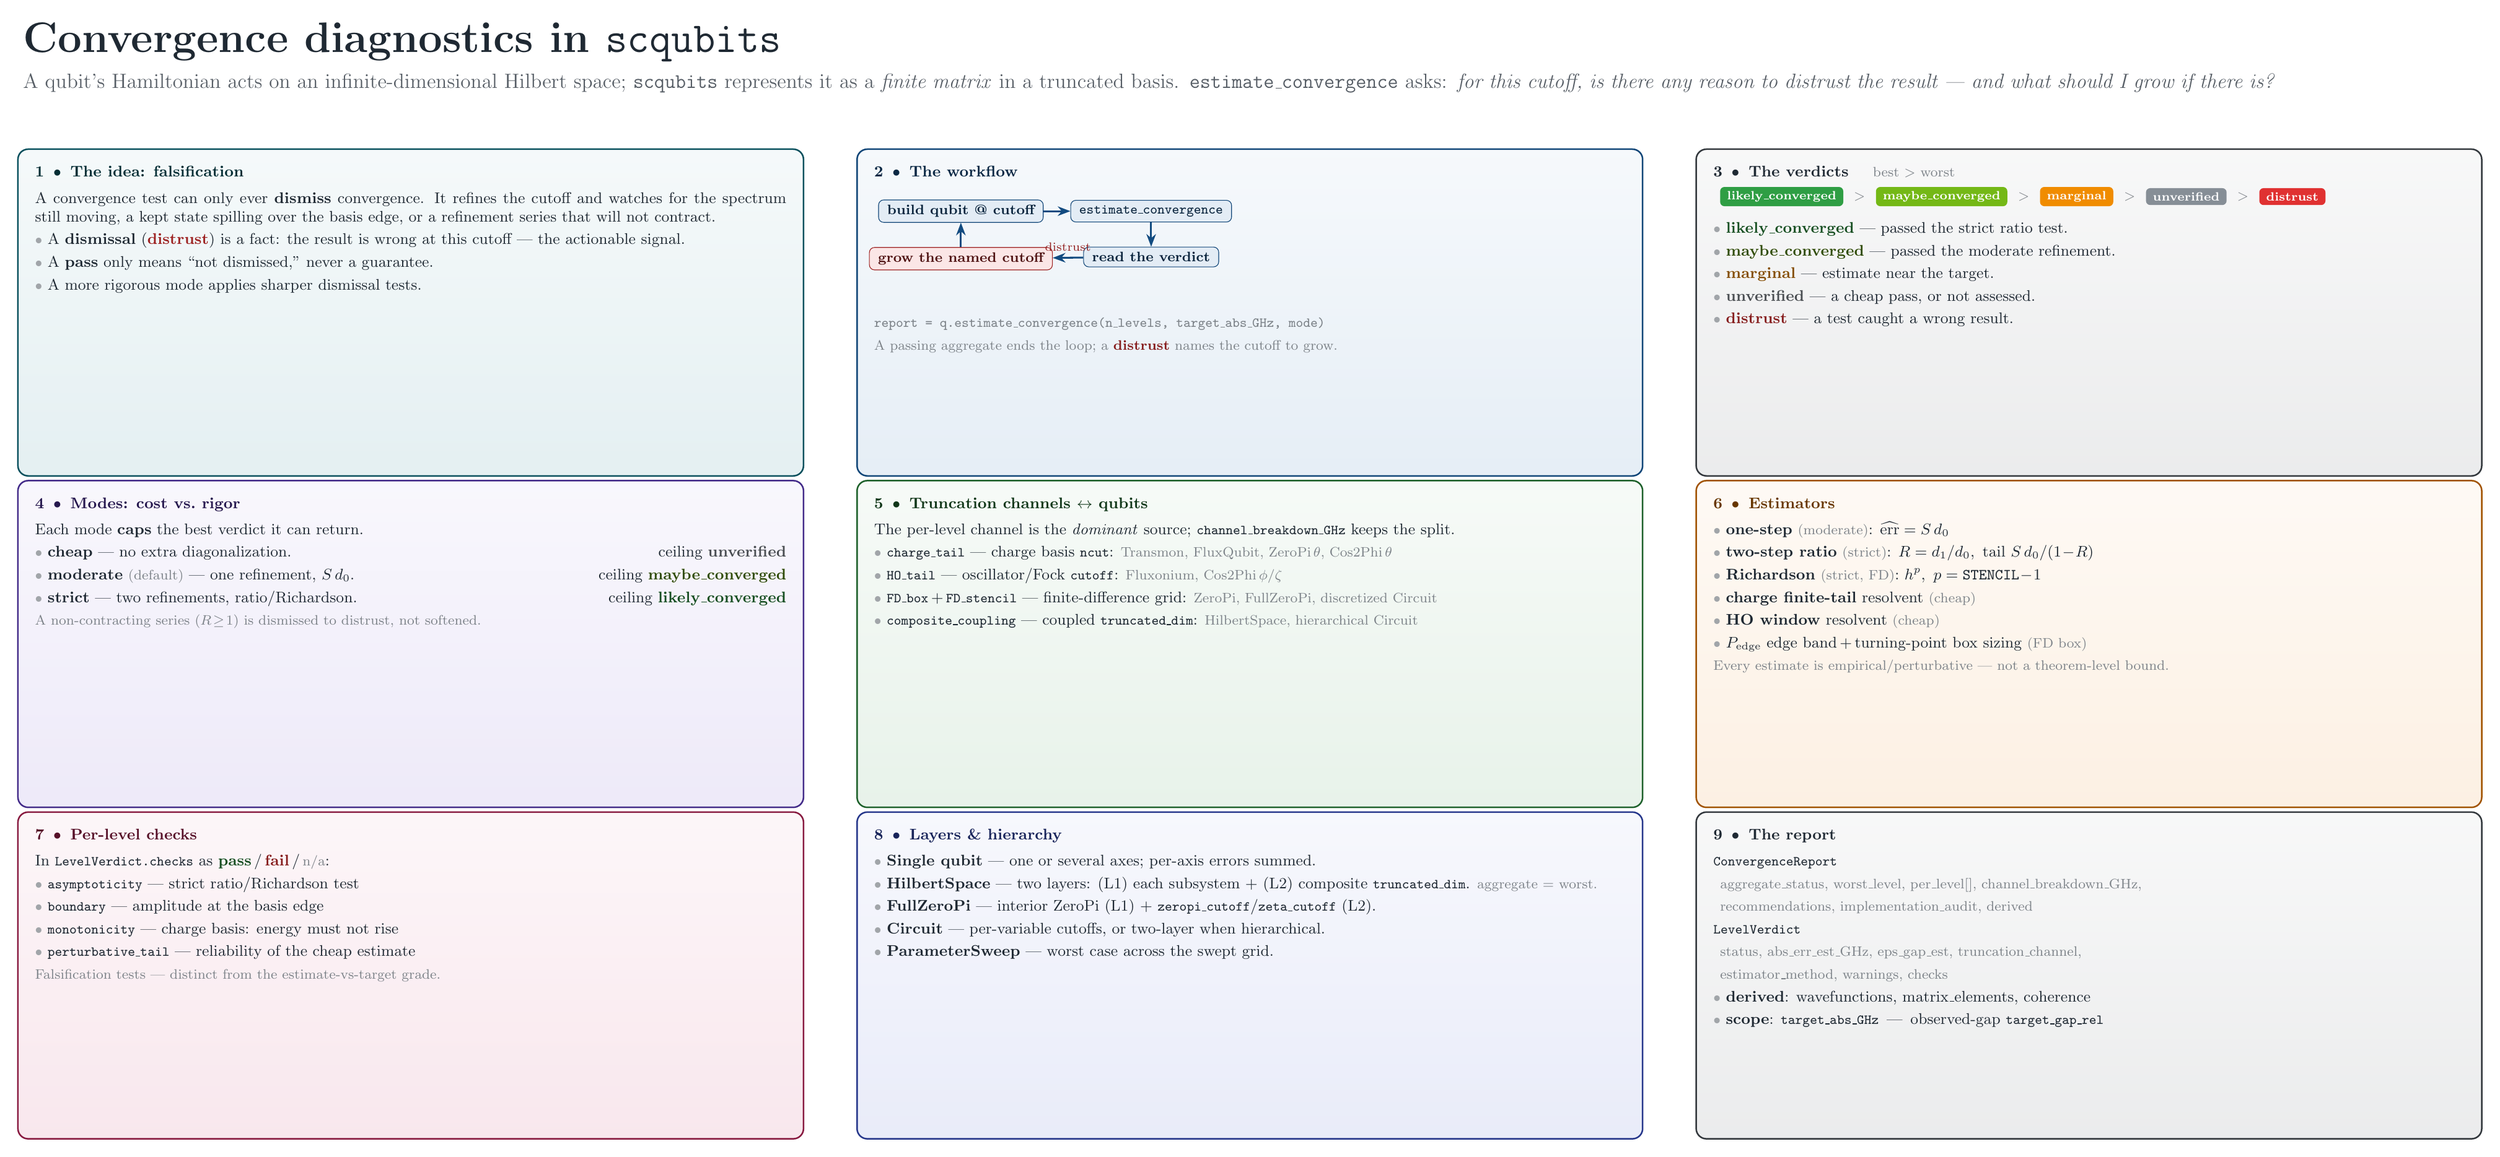
\begin{tikzpicture}

% ===================== TITLE =====================
\node[anchor=north west, text=ink] at (0,0)
  {\fontsize{30}{34}\selectfont\bfseries Convergence diagnostics in \texttt{scqubits}};
\node[anchor=north west, text=ink!75, font=\large, text width=49.8cm] at (0,-1.05)
  {A qubit's Hamiltonian acts on an infinite-dimensional Hilbert space; \texttt{scqubits} represents it as a \emph{finite matrix} in a truncated basis.
   \texttt{estimate\_convergence} asks: \emph{for this cutoff, is there any reason to distrust the result --- and what should I grow if there is?}};

% ===================== ROW 1 =====================
% A: philosophy
\node[zone=idea, anchor=north west] (A) at (\colA,\rowA) {\body{%
  \zt{idea!40!black}{1\, $\bullet$\, The idea: falsification}
  A convergence test can only ever \textbf{dismiss} convergence. It refines the
  cutoff and watches for the spectrum still moving, a kept state spilling over the
  basis edge, or a refinement series that will not contract.\par
  \bul A \textbf{dismissal} (\textcolor{vdist!70!black}{\bfseries distrust}) is a fact: the result is wrong at this cutoff --- the actionable signal.\par
  \bul A \textbf{pass} only means ``not dismissed,'' never a guarantee.\par
  \bul A more rigorous mode applies sharper dismissal tests.
}};

% B: workflow (loop drawn over reserved space, caption inside)
\node[zone=flow, anchor=north west] (B) at (\colB,\rowA) {\body{%
  \zt{flow!40!black}{2\, $\bullet$\, The workflow}
  \vspace{2.55cm}\par
  \bk{\cd{report = q.estimate\_convergence(n\_levels, target\_abs\_GHz, mode)}}\par
  \bk{A passing aggregate ends the loop; a \textcolor{vdist!60!black}{\bfseries distrust} names the cutoff to grow.}
}};
\node[pill=flow, anchor=north west] (w1) at ($(B.north west)+(0.45,-1.05)$) {build qubit @ cutoff};
\node[pill=flow, right=0.55cm of w1] (w2) {\cd{estimate\_convergence}};
\node[pill=flow, below=0.5cm of w2] (w3) {read the verdict};
\node[pill=vdist, below=0.5cm of w1] (w4) {grow the named cutoff};
\draw[fa] (w1) -- (w2);
\draw[fa] (w2) -- (w3);
\draw[fa] (w3) -- node[font=\scriptsize, text=vdist!65!black, above=0pt]{distrust} (w4);
\draw[fa] (w4) -- (w1);

% C: verdicts (one-line inequality + meanings)
\node[zone=repo, anchor=north west] (C) at (\colC,\rowA) {\body{%
  \zt{ink}{3\, $\bullet$\, The verdicts \quad\normalfont\bk{best $>$ worst}}
  \vspace{0.62cm}\par
  \bul \textcolor{vlikely!50!black}{\bfseries likely\_converged} --- passed the strict ratio test.\par
  \bul \textcolor{vmaybe!42!black}{\bfseries maybe\_converged} --- passed the moderate refinement.\par
  \bul \textcolor{vmarg!55!black}{\bfseries marginal} --- estimate near the target.\par
  \bul \textcolor{vunver!55!black}{\bfseries unverified} --- a cheap pass, or not assessed.\par
  \bul \textcolor{vdist!60!black}{\bfseries distrust} --- a test caught a wrong result.
}};
% one-line chip inequality, placed in the reserved strip near the top of C
\node[vchip=vlikely, anchor=base west] (k1) at ($(C.north west)+(0.5,-1.05)$) {likely\_converged};
\node[gt, right=2.5pt of k1] (s1) {$>$};
\node[vchip=vmaybe, right=2.5pt of s1] (k2) {maybe\_converged};
\node[gt, right=2.5pt of k2] (s2) {$>$};
\node[vchip=vmarg, right=2.5pt of s2] (k3) {marginal};
\node[gt, right=2.5pt of k3] (s3) {$>$};
\node[vchip=vunver, right=2.5pt of s3] (k4) {unverified};
\node[gt, right=2.5pt of k4] (s4) {$>$};
\node[vchip=vdist, right=2.5pt of s4] (k5) {distrust};

% ===================== ROW 2 =====================
% D: modes
\node[zone=mode, anchor=north west] (D) at (\colA,\rowB) {\body{%
  \zt{mode!40!black}{4\, $\bullet$\, Modes: cost vs.\ rigor}
  Each mode \textbf{caps} the best verdict it can return.\par
  \bul \textbf{cheap} --- no extra diagonalization. \hfill ceiling \textcolor{vunver!55!black}{\bfseries unverified}\par
  \bul \textbf{moderate} \bk{(default)} --- one refinement, $S\,d_0$. \hfill ceiling \textcolor{vmaybe!42!black}{\bfseries maybe\_converged}\par
  \bul \textbf{strict} --- two refinements, ratio/Richardson. \hfill ceiling \textcolor{vlikely!50!black}{\bfseries likely\_converged}\par
  \bk{A non-contracting series ($R\!\ge\!1$) is dismissed to distrust, not softened.}
}};

% E: channels <-> qubits
\node[zone=chan, anchor=north west] (E) at (\colB,\rowB) {\body{%
  \zt{chan!40!black}{5\, $\bullet$\, Truncation channels $\leftrightarrow$ qubits}
  The per-level channel is the \emph{dominant} source; \cd{channel\_breakdown\_GHz} keeps the split.\par
  \bul \cd{charge\_tail} --- charge basis \cd{ncut}: \bk{Transmon, FluxQubit, ZeroPi\,$\theta$, Cos2Phi\,$\theta$}\par
  \bul \cd{HO\_tail} --- oscillator/Fock \cd{cutoff}: \bk{Fluxonium, Cos2Phi\,$\phi/\zeta$}\par
  \bul \cd{FD\_box}\,+\,\cd{FD\_stencil} --- finite-difference grid: \bk{ZeroPi, FullZeroPi, discretized Circuit}\par
  \bul \cd{composite\_coupling} --- coupled \cd{truncated\_dim}: \bk{HilbertSpace, hierarchical Circuit}\par
}};

% F: estimators
\node[zone=esti, anchor=north west] (F) at (\colC,\rowB) {\body{%
  \zt{esti!45!black}{6\, $\bullet$\, Estimators}
  \bul \textbf{one-step} \bk{(moderate)}: $\widehat{\mathrm{err}}=S\,d_0$\par
  \bul \textbf{two-step ratio} \bk{(strict)}: $R=d_1/d_0$,\, tail $S\,d_0/(1\!-\!R)$\par
  \bul \textbf{Richardson} \bk{(strict, FD)}: $h^{p}$,\, $p=\texttt{STENCIL}\!-\!1$\par
  \bul \textbf{charge finite-tail} resolvent \bk{(cheap)}\par
  \bul \textbf{HO window} resolvent \bk{(cheap)}\par
  \bul $P_{\rm edge}$ edge band\,+\,turning-point box sizing \bk{(FD box)}\par
  \bk{Every estimate is empirical/perturbative --- not a theorem-level bound.}
}};

% ===================== ROW 3 =====================
% G: checks
\node[zone=chek, anchor=north west] (G) at (\colA,\rowC) {\body{%
  \zt{chek!45!black}{7\, $\bullet$\, Per-level checks}
  In \cd{LevelVerdict.checks} as \textcolor{vlikely!50!black}{\bfseries pass}\,/\,\textcolor{vdist!60!black}{\bfseries fail}\,/\,\bk{n/a}:\par
  \bul \cd{asymptoticity} --- strict ratio/Richardson test\par
  \bul \cd{boundary} --- amplitude at the basis edge\par
  \bul \cd{monotonicity} --- charge basis: energy must not rise\par
  \bul \cd{perturbative\_tail} --- reliability of the cheap estimate\par
  \bk{Falsification tests --- distinct from the estimate-vs-target grade.}
}};

% H: hierarchy
\node[zone=hier, anchor=north west] (H) at (\colB,\rowC) {\body{%
  \zt{hier!45!black}{8\, $\bullet$\, Layers \& hierarchy}
  \bul \textbf{Single qubit} --- one or several axes; per-axis errors summed.\par
  \bul \textbf{HilbertSpace} --- two layers: (L1) each subsystem $+$ (L2) composite \cd{truncated\_dim}. \bk{aggregate = worst.}\par
  \bul \textbf{FullZeroPi} --- interior ZeroPi (L1) $+$ \cd{zeropi\_cutoff}/\cd{zeta\_cutoff} (L2).\par
  \bul \textbf{Circuit} --- per-variable cutoffs, or two-layer when hierarchical.\par
  \bul \textbf{ParameterSweep} --- worst case across the swept grid.\par
}};

% I: report
\node[zone=repo, anchor=north west] (I) at (\colC,\rowC) {\body{%
  \zt{ink}{9\, $\bullet$\, The report}
  \cd{ConvergenceReport}\par
  \hspace{4pt}\bk{aggregate\_status, worst\_level, per\_level[], channel\_breakdown\_GHz,}\par
  \hspace{4pt}\bk{recommendations, implementation\_audit, derived}\par
  \cd{LevelVerdict}\par
  \hspace{4pt}\bk{status, abs\_err\_est\_GHz, eps\_gap\_est, truncation\_channel,}\par
  \hspace{4pt}\bk{estimator\_method, warnings, checks}\par
  \bul \textbf{derived}: wavefunctions, matrix\_elements, coherence\par
  \bul \textbf{scope}: \cd{target\_abs\_GHz} \,|\, observed-gap \cd{target\_gap\_rel}\par
}};

\end{tikzpicture}
\end{document}
